\documentclass[10pt]{beamer}

\setbeamersize{text margin left=0.5cm, text margin right=0.5cm}

\usepackage{alltt}%
%\usetheme{Boadilla}
\usetheme[progressbar = foot, background=light]{metropolis} 
%\useoutertheme{split}

%\usepackage{listings}
\makeatletter
\def\maxwidth{ %
  \ifdim\Gin@nat@width>\linewidth
    \linewidth
  \else
    \Gin@nat@width
  \fi
}
\makeatother

\definecolor{fgcolor}{rgb}{0.345, 0.345, 0.345}
\newcommand{\hlnum}[1]{\textcolor[rgb]{0.686,0.059,0.569}{#1}}%
\newcommand{\hlstr}[1]{\textcolor[rgb]{0.192,0.494,0.8}{#1}}%
\newcommand{\hlcom}[1]{\textcolor[rgb]{0.678,0.584,0.686}{\textit{#1}}}%
\newcommand{\hlopt}[1]{\textcolor[rgb]{0,0,0}{#1}}%
\newcommand{\hlstd}[1]{\textcolor[rgb]{0.345,0.345,0.345}{#1}}%
\newcommand{\hlkwa}[1]{\textcolor[rgb]{0.161,0.373,0.58}{\textbf{#1}}}%
\newcommand{\hlkwb}[1]{\textcolor[rgb]{0.69,0.353,0.396}{#1}}%
\newcommand{\hlkwc}[1]{\textcolor[rgb]{0.333,0.667,0.333}{#1}}%
\newcommand{\hlkwd}[1]{\textcolor[rgb]{0.737,0.353,0.396}{\textbf{#1}}}%
\let\hlipl\hlkwb

\usepackage{framed}
\makeatletter
\newenvironment{kframe}{%
 \def\at@end@of@kframe{}%
 \ifinner\ifhmode%
  \def\at@end@of@kframe{\end{minipage}}%
  \begin{minipage}{\columnwidth}%
 \fi\fi%
 \def\FrameCommand##1{\hskip\@totalleftmargin \hskip-\fboxsep
 \colorbox{shadecolor}{##1}\hskip-\fboxsep
     % There is no \\@totalrightmargin, so:
     \hskip-\linewidth \hskip-\@totalleftmargin \hskip\columnwidth}%
 \MakeFramed {\advance\hsize-\width
   \@totalleftmargin\z@ \linewidth\hsize
   \@setminipage}}%
 {\par\unskip\endMakeFramed%
 \at@end@of@kframe}
\makeatother

\definecolor{shadecolor}{rgb}{.97, .97, .97}
\definecolor{messagecolor}{rgb}{0, 0, 0}
\definecolor{warningcolor}{rgb}{1, 0, 1}
\definecolor{errorcolor}{rgb}{1, 0, 0}
\newenvironment{knitrout}{}{} % an empty environment to be redefined in TeX


\usepackage[utf8]{inputenc}
\usepackage{default}

\usepackage{xcolor}%for color mixing

\usepackage{amsmath}%
\usepackage{amsfonts}%
\usepackage{amssymb}%
\usepackage{graphicx}

\usepackage{tikz}
\usepackage{multirow}
\usepackage{booktabs}

\setbeamertemplate{itemize/enumerate body begin}{\small}

%%%%%%%%%%%%%%%%%%%%%%%%%%%%%%%%%%%%%%%%%%%%%%%%%%%%%%%%%%%%%%%%%%%%%%%%%%%%%%%%%%

\title{Statistical Modelling: Understanding Variance/Error Structure}
\subtitle{Chapter 4}
\author{Terry Neeman and Timoth\'ee Bonnet}
\date{\today}

\begin{document}

%\lstset{language=R}%code

\AtBeginSection[]
{
  \begin{frame}<beamer>
    \frametitle{}
    \tableofcontents[currentsection,sectionstyle=show/show,subsectionstyle=show/shaded/hide]% down vote\tableofcontents[currentsection,currentsubsection,hideothersubsections,sectionstyle=show/hide,subsectionstyle=show/shaded/hide] 
  \end{frame}
}


\begin{frame}{}
\maketitle

\end{frame}
%%%%%%%%%%%%%%%%%%%%%%%

\begin{frame}{Statistical models: MEAN and VARIANCE components}
\centering
  ${\color{purple}{response}} = \underbrace{{\color{blue}{A}} + {\color{red}{D}} \times {\color{orange}{predictor}}}_{\substack{\text{Mean Structure} \\ \text{Experimental factors}}} + 
  \underbrace{{\color{gray}{\epsilon}}, \text{ with } {\color{gray}{\epsilon \sim N(0,\sigma)}}}_{\substack{\text{Variance Structure} \\ \text{Unrelated to experiment factors} \\ \text{Unexplained ``noise''}}}$

  \pause 
  \vfill
  
  What is in ${\color{gray}{\epsilon}}$? How can we tweak that? Why should we care?
  \end{frame}
%%%%%%%%%%%%

\begin{frame}{Describe the data structure in this experiment}
 
 How is seedling emergence (in Banksia) influenced by temperature and moisture?
 
 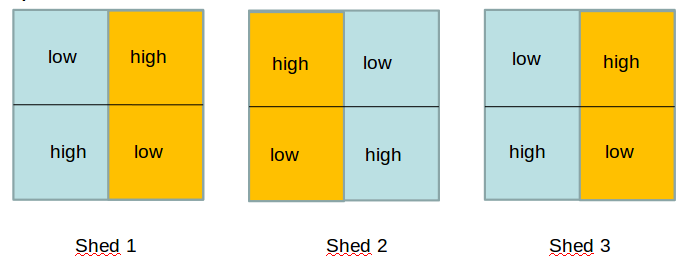
\includegraphics[width=0.9\textwidth]{Figures/banksiashed}


Set up: 3 sheds, 4 garden beds per shed, 24 pots per bed.\\
Experimental factors:  2 temperatures, 2 water levels

\end{frame}
%%%%%%%%%%%

\begin{frame}{Key components of a statistical model of an experiment}
 \begin{itemize}
  \item Outcome measure
  \begin{itemize}
   \item Plant height at week 3
    \item Number of leaves at week 3
  \end{itemize}
  \item Experimental factors 
  \begin{itemize}
   \item Temperature (warm/ control)
    \item Watering conditions (low/high) 
    \item Question: how does each factor affect outcome measures? Do the factors interact?
  \end{itemize}
  \item \textbf{Blocking factors}
  \begin{itemize}
   \item Shed
    \item “half-shed” within Shed
    \item Garden bed within “half-shed”
  \end{itemize}
\end{itemize}
\end{frame}
%%%%%%%%%%%%

\begin{frame}{Message 1: A small p-value is not always evidence of a treatment effect}

  \begin{columns}
    \begin{column}{0.5\textwidth}
	\begin{center}
	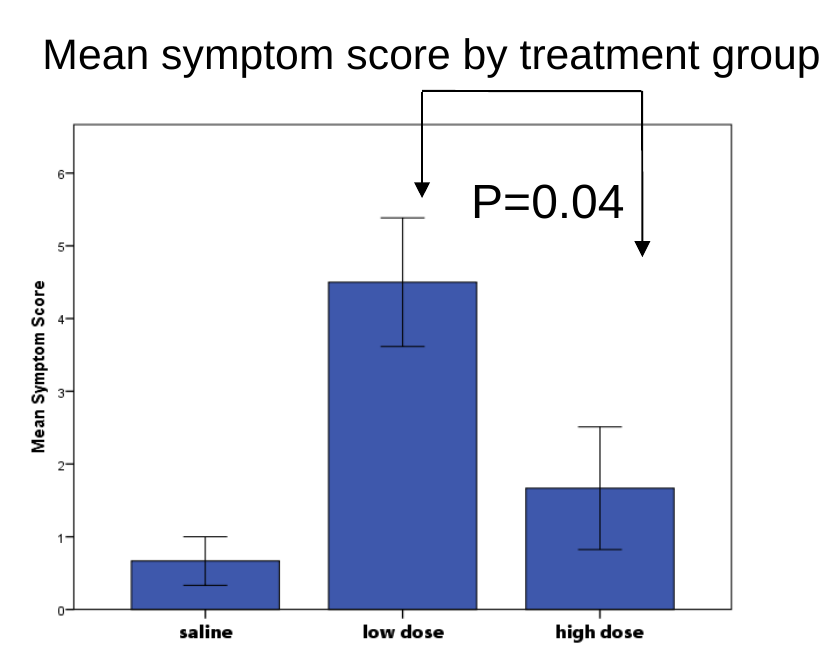
\includegraphics[width=\textwidth]{Figures/message1}
	\end{center}
    \end{column}
    
    \begin{column}{0.5\textwidth}
    \begin{block}{Vaccine challenge experiment:}
      \begin{itemize} 
       \item 6 mice/group (saline/low dose/high dose)
       \item All mice challenged with Shigella
       \item Followed for 14 days
       \item  Outcome: Symptom score average Days 2 - 8
      \end{itemize}
      \end{block}
      
      \begin{alertblock}{}
       One-way ANOVA (post-hoc Bonferroni) p=0.04
      \end{alertblock}

    \end{column}
  \end{columns}
  

\end{frame}
%%%%%%%%%%%%%%%%%%%%%%%


\begin{frame}{ Noise confounded with treatment}

 \begin{center}
  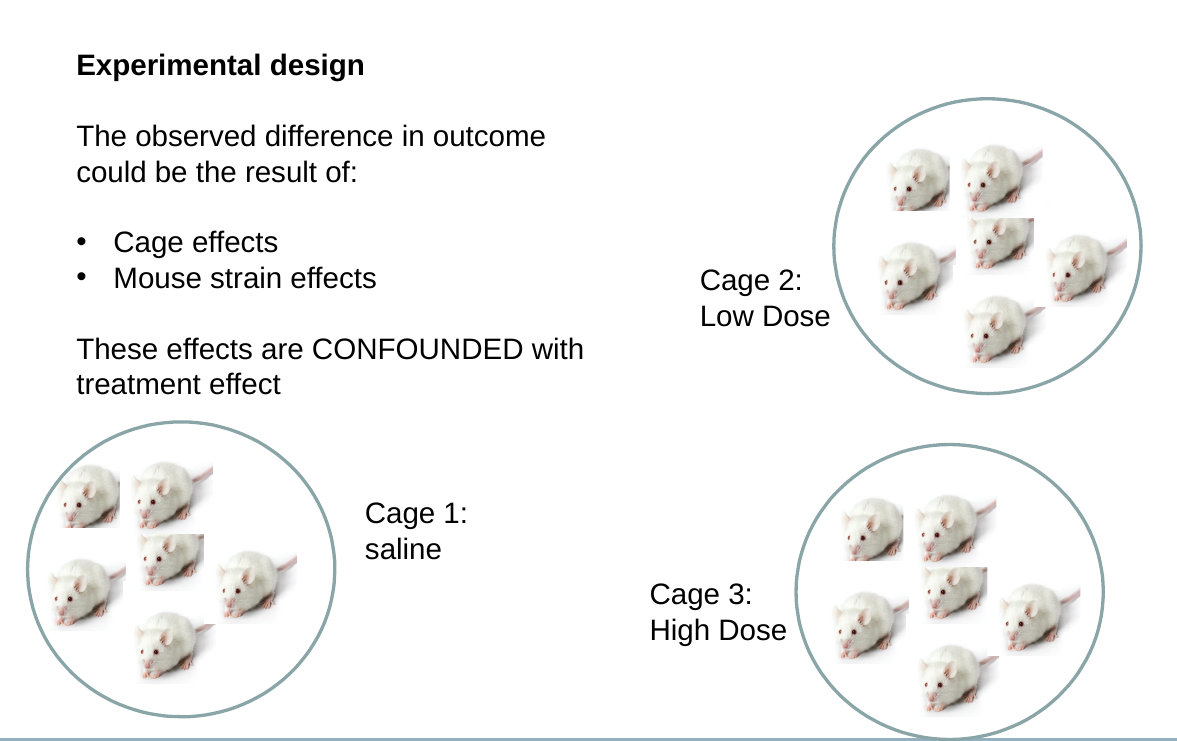
\includegraphics[width=0.7\textwidth]{Figures/mice}
 \end{center}
 
 \pause
 
 \begin{block}{Solutions:}
  Mixed cages: can compare within cages \\
  More cages: must compare between cages 
 \end{block}

\end{frame}
%%%%%%%%%%%

\begin{frame}{ Noise confounded with treatment}

  \begin{block}{Mixed cages: can compare within cages}
    \begin{itemize}
     \item \textbf{Share the noise among treatments}
     \item Few cages needed: Technically efficient
     \item But may be technically impossible
    \end{itemize}
  \end{block}

 \pause
 
 \begin{block}{More cages: must compare between cages }
    \begin{itemize}
    \item \textbf{Redefine experimental unit}
    \item Noise among cages, instead of within
    \item Needs to re-scale the experiment
    \end{itemize} 
 \end{block}

\end{frame}
%%%%%%%%%%%

\begin{frame}{Is photosynthetic rate affected by temperature?}

 \begin{block}{Research context}
 \begin{columns}
  \begin{column}{0.8\textwidth}
   \begin{itemize}
    \item Outcome measure: Photosynthetic rate
    \item Experimental factors: Temperature (high/low)
    \item Blocking factors: Position (4)
   \end{itemize}
  \end{column}
  \begin{column}{0.2\textwidth}
    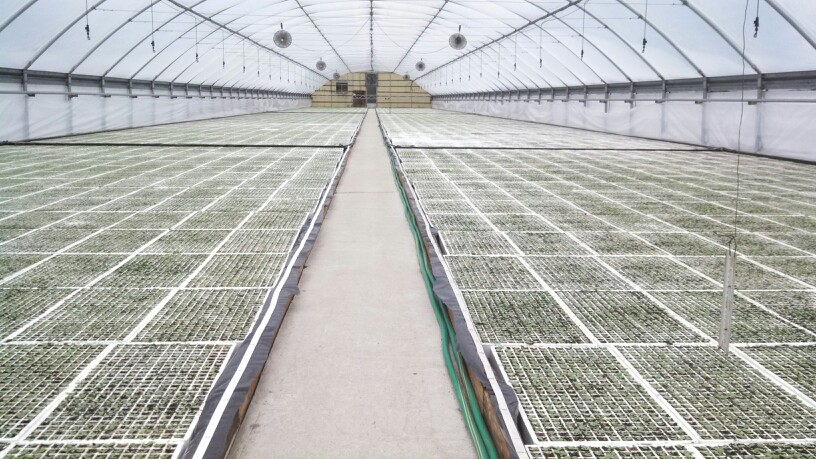
\includegraphics[width=0.9\textwidth]{Figures/photos}
  \end{column}

 \end{columns}
 \end{block}
 
 \textbf{How many parameters?}
 
\pause

2 parameters to describe the effect of temperatures \\

\pause

+ some to correct for blocking factors
 
\end{frame}
%%%%%%%%%%%

\begin{frame}[fragile]{Inference using linear model without and with blocking in R}
 
 Without blocking
  \begin{knitrout}
\definecolor{shadecolor}{rgb}{0.969, 0.969, 0.969}\color{fgcolor}\begin{kframe}
\begin{verbatim}
m_noblock <- lm(PhotoRate~Temp, data=photo)
anova(m_noblock)
\end{verbatim}
\end{kframe}
\end{knitrout}

\begin{knitrout}
\definecolor{shadecolor}{rgb}{0.9, 0.9, 0.969}\color{fgcolor}\begin{kframe}
\begin{verbatim}
Analysis of Variance Table
 
Response: PhotoRate
          		Df  Sum Sq 	Mean Sq 	F value 	Pr(>F)
Temp      	1       613.3  	  613.28  	0.4386 	0.5147
Residuals           22   30760.8 	1398.22
\end{verbatim}
\end{kframe}
\end{knitrout}
 
\end{frame}
%%%%%%%%%%%


\begin{frame}[fragile]{Inference using linear model without and with blocking in R}
 
 Blocking with a fixed factor
  \begin{knitrout}
\definecolor{shadecolor}{rgb}{0.969, 0.969, 0.969}\color{fgcolor}\begin{kframe}
\begin{verbatim}
m_block <- lm(PhotoRate~Temp+ as.factor(Position), data=photo)
anova(m_block)
\end{verbatim}
\end{kframe}
\end{knitrout}

\begin{knitrout}
\definecolor{shadecolor}{rgb}{0.9, 0.9, 0.969}\color{fgcolor}\begin{kframe}
\begin{verbatim}
Analysis of Variance Table

Response: PhotoRate
                    Df  Sum Sq Mean Sq F value    Pr(>F)    
Temp                 1   613.3   613.3   4.521   0.04681 *  
as.factor(Position)  3 28183.4  9394.5  69.253 2.047e-10 ***
Residuals           19  2577.4   135.7                      
---
Signif. codes:  0 ‘***’ 0.001 ‘**’ 0.01 ‘*’ 0.05 ‘.’ 0.1 ‘ ’ 1
\end{verbatim}
\end{kframe}
\end{knitrout}
 
 \textbf{Clearer evidence for an effect of temperature with blocking}
 
\end{frame}
%%%%%%%%%%%


\begin{frame}[fragile]{Inference using linear model without and with blocking in R}
 
 Blocking with a \textbf{random effect}
  \begin{knitrout}
\definecolor{shadecolor}{rgb}{0.969, 0.969, 0.969}\color{fgcolor}\begin{kframe}
\begin{verbatim}
library(lme4)
library(lmerTest)
m_block_re <- lmer(PhotoRate~Temp+ (1|Position), data=photo)
anova(m_block_re)
\end{verbatim}
\end{kframe}
\end{knitrout}

\begin{knitrout}
\definecolor{shadecolor}{rgb}{0.9, 0.9, 0.969}\color{fgcolor}\begin{kframe}
\begin{verbatim}
Type III Analysis of Variance Table with Satterthwaite's method
     Sum Sq Mean Sq NumDF DenDF F value  Pr(>F)  
Temp 613.28  613.28     1    19   4.521 0.04681 *
---
Signif. codes:  0 ‘***’ 0.001 ‘**’ 0.01 ‘*’ 0.05 ‘.’ 0.1 ‘ ’ 1
\end{verbatim}
\end{kframe}
\end{knitrout}
 
 \textbf{Clearer evidence for an effect of temperature with blocking}
 
\end{frame}
%%%%%%%%%%%

\begin{frame}[fragile]{Try it in R}

1. Load data ``Prac4photosynthesis.csv''

2. Visualize the data

3. Model data and interpret output
\begin{knitrout}
\definecolor{shadecolor}{rgb}{0.969, 0.969, 0.969}\color{fgcolor}\begin{kframe}
\begin{verbatim}
library(lmerTest)
library(emmeans)
lmer1<-lmer(PhotoRate~Temp+(1|Position), data=photo)
anova(lmer1)
summary(lmer1)
emmeans(lmer1,~Temp)
\end{verbatim}
\end{kframe}
\end{knitrout}

4. Assess model assumptions
\begin{knitrout}
\definecolor{shadecolor}{rgb}{0.969, 0.969, 0.969}\color{fgcolor}\begin{kframe}
\begin{verbatim}
plot(lmer1)
\end{verbatim}
\end{kframe}
\end{knitrout}


\end{frame}
%%%%%%%%%%%



\begin{frame}{Fixed or random effect?}
  \begin{block}{In this example}
   \begin{itemize}
    \item Doesn't change inference (same p-value for temperature)
    \item Summary cleaner with random effect
   \end{itemize}
  \end{block}

  \pause
  
  \begin{block}{In general}
   \begin{itemize}
    \item Generally doesn't change inference much. Random effect slightly more efficient.
    \item Summary cleaner with random effect, especially when many random levels
    \item Random shifts the focus from level values to variation among levels
    \item Variance parameters interesting in themselves
    \item Are levels of interest (fixed) or are they some kind of noise (random)
   \end{itemize}
  \end{block}

\end{frame}
%%%%%%%%%%%%


\begin{frame}{Can a gene KO Arabidopsis modulate leaf temperature during drought?}
 \centering
 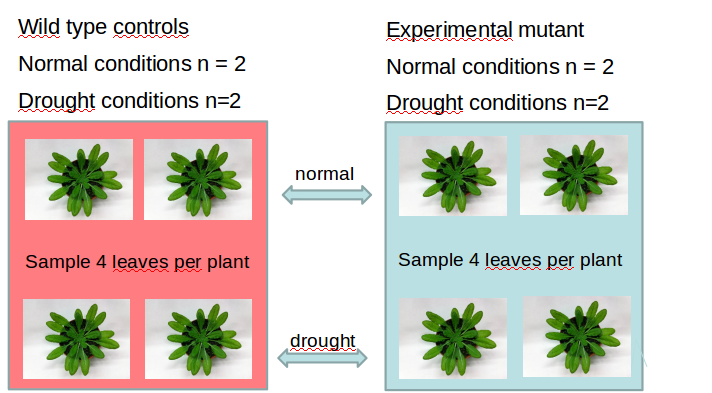
\includegraphics[width=0.9\textwidth]{Figures/koara}
\end{frame}
%%%%%%%%%%%


\begin{frame}{Visualising temperature data by treatment and Genotype}
 \begin{center}
 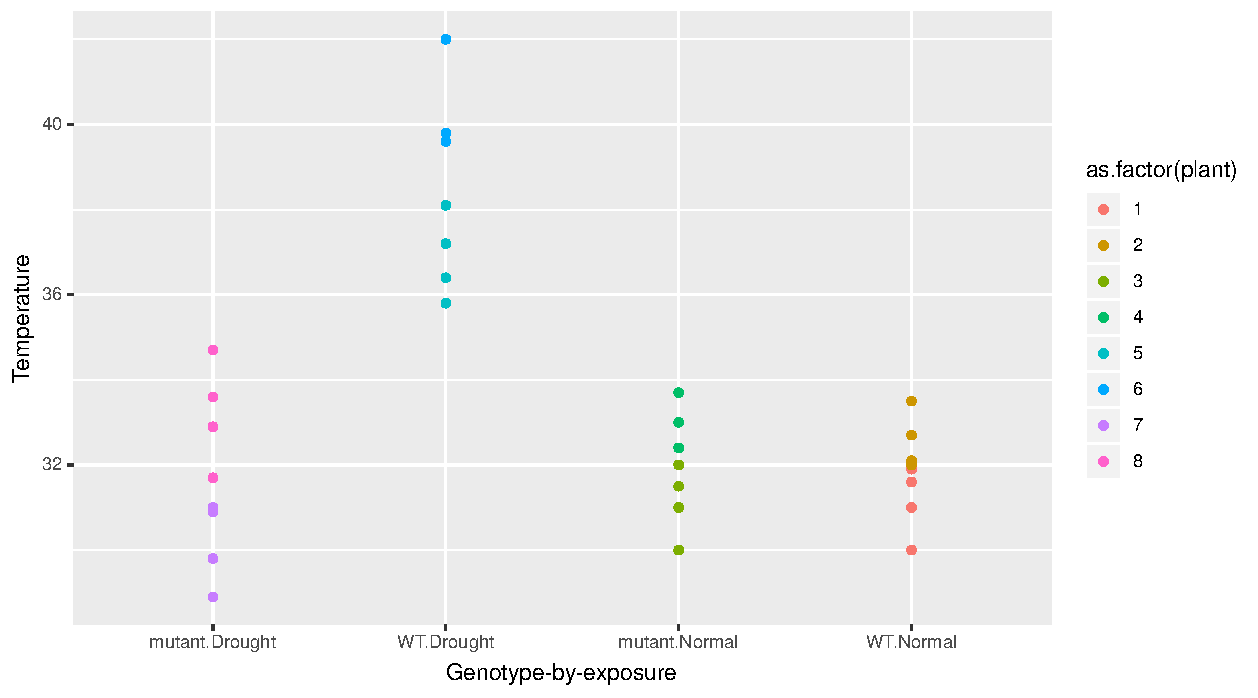
\includegraphics[width=0.9\textwidth]{Figures/droughtdata}
 \end{center}
 Outcome measure: Temperature\\
Experimental factors: Genotype (2), Watering conditions (2)\\
Blocking factor: Plant 
\end{frame}
%%%%%%%%%%%

\begin{frame}[fragile]{Set up analysis for this experiment}
 \begin{knitrout}
 \footnotesize
\definecolor{shadecolor}{rgb}{0.969, 0.969, 0.969}\color{fgcolor}\begin{kframe}
\begin{verbatim}
drought <- read.csv("Data/Prac3droughtdata.csv")
str(drought)

#Make Plant a Factor
drought$plant<- factor(drought$plant)

#Set Reference Levels
drought$Genotype<-relevel(drought$Genotype, ref="WT")
drought$WaterCondition<-relevel(drought$WaterCondition, ref="Normal")

ggplot(drought, aes(x=interaction(Genotype, WaterCondition),
		     y=Temperature, color=plant))+
  geom_point()+xlab("Genotype-by-exposure")
\end{verbatim}
\end{kframe}
\end{knitrout}

\end{frame}
%%%%%%%%%%%%

\begin{frame}[fragile]{Analysis of Variance without and with variance structure in R}
 
 \pause 
  \begin{knitrout}
 \footnotesize
\definecolor{shadecolor}{rgb}{0.969, 0.969, 0.969}\color{fgcolor}\begin{kframe}
\begin{verbatim}
 lm.drought <- lm(Temperature ~ Genotype*WaterCondition, data=drought)
anova(lm.drought)

\end{verbatim}
\end{kframe}
\end{knitrout}
\pause
  \begin{knitrout}
 \footnotesize
\definecolor{shadecolor}{rgb}{0.9, 0.9, 0.969}\color{fgcolor}\begin{kframe}
\begin{verbatim}
                        Df  Sum Sq Mean Sq F value    Pr(>F)    
Genotype                 1  89.111  89.111  33.289 3.407e-06 ***
WaterCondition           1  80.645  80.645  30.127 7.304e-06 ***
Genotype:WaterCondition  1 101.531 101.531  37.929 1.195e-06 ***
\end{verbatim}
\end{kframe}
\end{knitrout}

\pause
 \begin{knitrout}
 \footnotesize
\definecolor{shadecolor}{rgb}{0.969, 0.969, 0.969}\color{fgcolor}\begin{kframe}
\begin{verbatim}
lmer.drought <- lmer(Temperature ~ Genotype*WaterCondition + (1|plant),
data=drought)
anova(lmer.drought)
\end{verbatim}
\end{kframe}
\end{knitrout}

  \begin{knitrout}
 \footnotesize
\definecolor{shadecolor}{rgb}{0.9, 0.9, 0.969}\color{fgcolor}\begin{kframe}
\begin{verbatim}
                        Sum Sq Mean Sq NumDF DenDF F value  Pr(>F)  
Genotype                5.8403  5.8403     1     4  6.6257 0.06171 .
WaterCondition          5.2854  5.2854     1     4  5.9962 0.07054 .
Genotype:WaterCondition 6.6543  6.6543     1     4  7.5491 0.05150 .
\end{verbatim}
\end{kframe}
\end{knitrout}
 
\end{frame}
%%%%%%%%%%%%

\begin{frame}[fragile]{Treatment effect estimates without and with variance structure}
   \begin{knitrout}
 \footnotesize
\definecolor{shadecolor}{rgb}{0.969, 0.969, 0.969}\color{fgcolor}\begin{kframe}
\begin{verbatim}
emmeans(lm.drought,~Genotype*WaterCondition) 
\end{verbatim}
\end{kframe}
\end{knitrout}

  \begin{knitrout}
 \footnotesize
\definecolor{shadecolor}{rgb}{0.9, 0.9, 0.969}\color{fgcolor}\begin{kframe}
\begin{verbatim}
Genotype Condition  emmean    SE  df 	lower.CL upper.CL 
WT       Normal      31.85  0.578 28 	30.66 		33.03 
WT       Drought     38.58  0.578 28 	37.40 		39.77 
mutant   Normal      32.07  0.578 28 	30.89 		33.25 
mutant   Drought     31.68  0.578 28 	30.50 		32.87 
\end{verbatim}
\end{kframe}
\end{knitrout}


   \begin{knitrout}
 \footnotesize
\definecolor{shadecolor}{rgb}{0.969, 0.969, 0.969}\color{fgcolor}\begin{kframe}
\begin{verbatim}
emmeans(lmer.drought,~Genotype*WaterCondition)
\end{verbatim}
\end{kframe}
\end{knitrout}

  \begin{knitrout}
 \footnotesize
\definecolor{shadecolor}{rgb}{0.9, 0.9, 0.969}\color{fgcolor}\begin{kframe}
\begin{verbatim}
Genotype Condition emmean     SE  df   lower.CL upper.CL 
WT 	 Normal    31.85     1.29  4    28.25 	35.44 
WT 	 Drought   38.58     1.29  4    34.98 	42.18
mutant   Normal    32.07     1.29  4    28.47 	35.67  
mutant   Drought   31.68     1.29  4    28.08 	35.28
\end{verbatim}
\end{kframe}
\end{knitrout}

 \textbf{Correct blocking structure is essential for correct inference!}
\end{frame}
%%%%%%%%%%%%

\begin{frame}{Is dark respiration differentially affected by temperature between genotypes?}
  \begin{block}{Research context}
 \begin{columns}
  \begin{column}{0.8\textwidth}
   \begin{itemize}
      \item Outcome measure: Dark respiration
      \item Experimental factors:  Genotype (2) \& Temperature (4)
      \item Blocking factors:  Shelter (4) \&  Plants within shelter (20)

   \end{itemize}
  \end{column}
  \begin{column}{0.2\textwidth}
    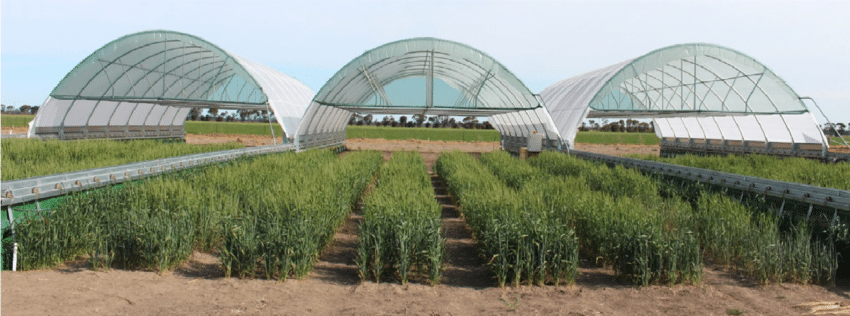
\includegraphics[width=0.9\textwidth]{Figures/darkresp}
  \end{column}

 \end{columns}
 \end{block}

8 parameter model (plus random effects)
 
 \end{frame}
%%%%%%%%%%%

\begin{frame}{Is dark respiration differentially affected by temperature between genotypes?}
 Analyse the data ``Prac4respiration data.csv''\\
 Answer the question\\
 Check assumptions\\
 Plot result
\end{frame}
%%%%%%%%%%%


\begin{frame}{Understanding different variance structure}
 
 \begin{center}
  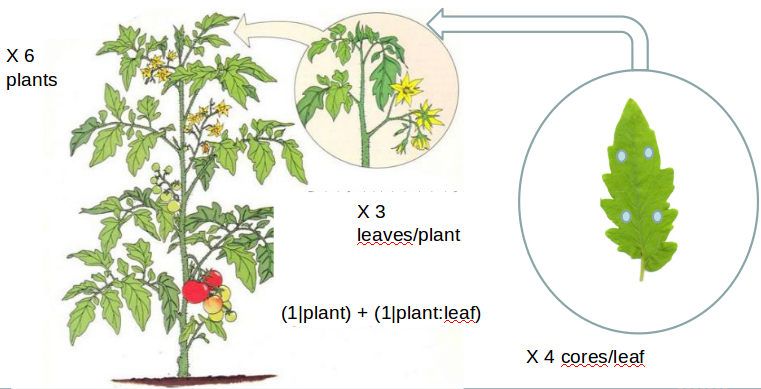
\includegraphics[width=0.9\textwidth]{Figures/nestedtomatoes}
 \end{center}

\end{frame}
%%%%%%%%%%%

\begin{frame}{Understanding different variance structure}
 
 \begin{center}
  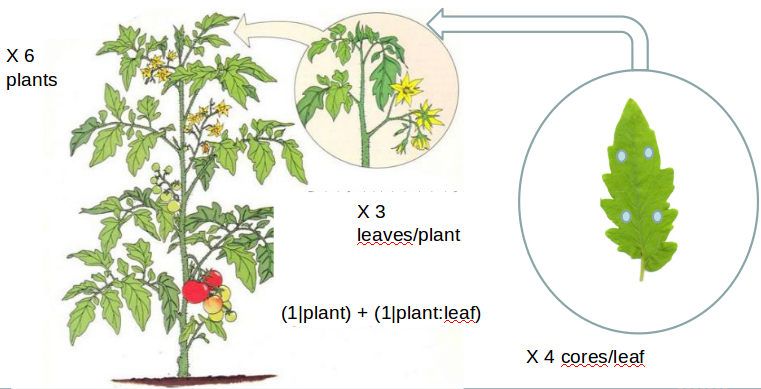
\includegraphics[width=0.9\textwidth]{Figures/nestedtomatoes}
 \end{center}

\end{frame}
%%%%%%%%%%%


\begin{frame}{Understanding different variance structure}
 
 \begin{center}
  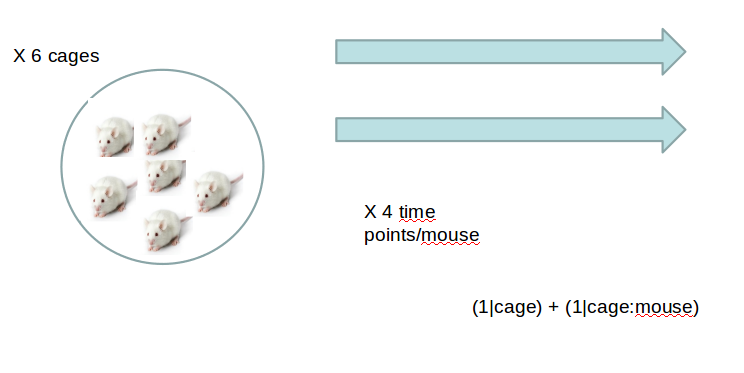
\includegraphics[width=0.9\textwidth]{Figures/nestedmice}
 \end{center}

\end{frame}
%%%%%%%%%%%

\begin{frame}{Understanding different variance structure: \textbf{Nested and Crossed structures}} 
\textbf{Crossed:} \texttt{(1|plate) + (1|row) + (1|column)}\\
\vspace{0.2cm}
\textbf{Nested:} \texttt{(1|plate) + (1|plate:row) + (1|plate:column) = (1|plate/row/column)}\\

What is the difference?

 \begin{center}
  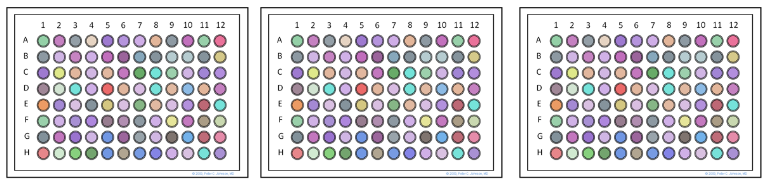
\includegraphics[width=0.9\textwidth]{Figures/nestedplates}
 \end{center}

 \textit{crossed random effects: one level of a random effect can appear in conjunction with more than one level of another random effect}
\end{frame}
%%%%%%%%%%%



\begin{frame}{Everything you need to know about mixed models}

\begin{itemize}
 \item \url{http://bbolker.github.io/mixedmodels-misc/glmmFAQ.html}
 \item Subscribe to mailing-list: \texttt{https://stat.ethz.ch/mailman/listinfo/r-sig-mixed-models}
\end{itemize}

\end{frame}
%%%%%%%%%%%%%


\begin{frame}{Summary of Statistical Modelling}
 \begin{alertblock}{Take-home}
  \begin{itemize}[<+->]
   \item Identify Statistical Framework of Experiment
    \begin{enumerate}
     \item Outcome measure
     \item Experimental factors
     \item Blocking factors
    \end{enumerate}
  \item Visualize data
  \item Try simple models first
  \item Assess model fit/assumptions
  \item interpret
  \end{itemize}

 \end{alertblock}

 
\end{frame}
%%%%%%%%%%%%

\end{document}
